\section{Absorption across channels}\label{sec:17.2}

A dark photon of \SI{25}{\micro eV} is absorbed by the tunneling atoms of an oxide film, one of \SI{36}{meV} by a longitudinal optical phonon of GaAs, and one of \SI{16}{eV} by the plasmon of silicon. Three events in a kilogram and year need $\zeta = 2.4\times10^{-15}$, $2.9\times10^{-17}$ and $1.0\times10^{-17}$ for the three (\cref{we:16-tls-dp,sec:11.8-dp,sec:10.7-darkphoton}). The numbers come from three chapters, but each is \cref{eq:8.2-abs} evaluated at one point, $\vect{q} = \vect{p}_\phi$ of order $10^{-3}m_\phi$ and $\omega = m_\phi$, with the response of a different target. Unlike scattering, absorption leaves no kinematic freedom: the mass fixes the energy, and a target either has an excitation at that point or does not absorb. Comparing the channels is then a matter of coverage, of which material absorbs at each mass, and by how much the medium screens it. Below a few \si{\micro eV} a second question enters, since the quanta are then softer than the thermal energy of a readout at millikelvin temperatures, and the field must be measured as a wave.

\subsection{In-medium mixing across targets}\label{sec:17.2-mixing}

Each boson probes one response function at that point. The dark photon measures the loss function $L(m_\phi)$ of the total dielectric function, \cref{eq:10.7-dp}, and every excitation that carries charge enters through it: interband pairs, optical phonons, tunneling atoms, donors, Dirac pairs and quasiparticle pairs alike. The axion-like particle with its electron coupling measures the spin-current response, which for independent electrons without spin--orbit coupling is the optical conductivity $\sigma_1$, \cref{eq:10.7-alp}, and which in a superconductor becomes $\sigma_1^{\mathcal{J}}$ of \cref{eq:15.4-sJ}; in a magnet it reaches the uniform spin precession instead, \cref{eq:14.3-peak}. Its photon coupling in a static field $\vect{B}_0$ measures $\hat{\vect{B}}_0\cdot\Imag[-\varepsilon^{-1}]\cdot\hat{\vect{B}}_0$, the dark-photon response with $\zeta = g_{a\gamma\gamma}B_0/m_\phi$ (\cref{eq:10.7-alpB}). The scalar coupled to electrons measures the kinetic-energy row $S_{\mathcal{T}\mathcal{T}}$ in a crystal without a polar vector, \cref{eq:10.7-scalar}, and in a polar crystal the electrons that each nucleus carries, \cref{eq:11.8-G}. Per unit target mass the three rates are proportional to $L/\rho_T$, to $m_\phi\sigma_1/\rho_T$ and to $S_{\mathcal{T}\mathcal{T}}/(m_\phi^2\rho_T)$.

The dark photon, and the axion-like particle in a field, mix with the photon of the medium, and for them the mixing sets a ceiling. At fixed $\varepsilon_1$ the loss function $L = \varepsilon_2/(\varepsilon_1^2 + \varepsilon_2^2)$ is largest at $\varepsilon_2 = |\varepsilon_1|$, where $\partial L/\partial\varepsilon_2$ vanishes, so that
\begin{equation}
  L(m_\phi) \le \frac{1}{2\,|\varepsilon_1(m_\phi)|} .
  \label{eq:17.2-Lbound}
\end{equation}
A material absorbs a dark photon strongly only where $\varepsilon_1$ is small. Below its gap silicon has $\varepsilon_1 = 11.7$ at room temperature, so $L \le 0.043$, and the cold edge reaches $1.5\times10^{-6}$ at \SI{1.2}{eV} (\cref{we:13-darkphoton-edge}). Amorphous SiO$_2$, with $\varepsilon_r = 3.9$, allows 0.13, and its two-level systems give $L = \tan\delta_0/\varepsilon_r = 7.7\times10^{-5}$ for the loss tangent $\tan\delta_0 = 3\times10^{-4}$ of a thermal oxide (\cref{eq:16.7-dp}). The background constants of ZrTe$_5$, 20.75 to 308 along its three axes, cap the Dirac pairs at $0.024$ for the polarization along the axis with the smallest constant and at $0.0016$ along the axis with the largest. At \SI{1}{meV} the condensate of aluminum has $\varepsilon_1 = -1.5\times10^8$, so $L \le 3.3\times10^{-9}$, and the phonon-assisted pairs reach $2.4\times10^{-16}$ (\cref{we:15-holstein}). The large values of $L$ sit where $\varepsilon_1$ crosses zero, at the longitudinal modes. At the longitudinal optical phonon of GaAs the width of the line alone limits it, $L = 2\mathcal{I}_{\mathrm{pol}}/\pi\gamma_{\mathrm{L}} = 1.33$, with $\gamma_{\mathrm{L}}$ the width of the longitudinal line (\cref{sec:11.8-dp}); it is 7.9 at the top longitudinal line of sapphire, \SI{112.4}{meV}, and 4.49 at the plasmon of silicon, \SI{16.4}{eV}. The deepest minima of the dark-photon reach curves are longitudinal modes, with $\zeta \approx 10^{-17}$ for three events in a kilogram and year. The same mixing places the phonon line of a polar crystal at $\omega_{\mathrm{L}}$, not at the transverse frequency where $\varepsilon_2$ peaks: at $\omega_{\mathrm{T}} = \SI{33.62}{meV}$ GaAs has $L = 0.0054$.

Each target then carries its own version of the screening factor. The two-level systems of a glass are screened once by the static constant, through $1/\varepsilon_r$. Dilute donors are screened once by the host, a factor $1/\varepsilon_{\mathrm{host}}^2 = 1/130$ on the absorption of each donor, with the cold constant 11.4 of silicon (\cref{sec:16.5-absorption}). In a Dirac material the published rates omitted one power of the background constant, the screening by the remote bands. With it included, the reach in $\zeta$ weakens by the polarization average of $\varepsilon_{\mathrm{bg},ii}^{1/2}$, a factor of 6.3 to 6.4 for ZrTe$_5$ (\cref{sec:16.1}). A clean superconductor screens a field of \SI{1}{meV} by $1/|\varepsilon|^2 = 4.4\times10^{-17}$, and it reaches just $\zeta = 1.5\times10^{-9}$ with a kilogram and year. A magnet absorbs a dark photon through its magnetic field, which is smaller than the electric field by the speed $v$ (\cref{we:9-darkphoton}), and the field inside the sample depends on its dielectric constant and on the conductors around it (\cref{sec:14.3}).

The axion-like particle has no mixing, and the ceiling \cref{eq:17.2-Lbound} does not apply to it. As a result, the material that screens a dark photon most is among the best absorbers. Clean aluminum absorbs a particle of \SI{0.72}{meV} through the spin current, and three events in a kilogram and year need $g_{aee} = 6.1\times10^{-13}$ (\cref{sec:15.4}), the same order as the best that silicon reaches, $1.4\times10^{-13}$ at \SI{4.3}{eV}. The silicon optimum lies near the main peak of $\varepsilon_2$, the region of strongest suppression for the dark photon. The two bosons thus favor opposite regions of the same spectrum, the dark photon the zeros of $\varepsilon_1$ and the axion-like particle the maxima of $\varepsilon_2$, and the ratio of their rates at equal couplings is $(3m_\phi^2/4m_e^2e^2)|\varepsilon|^2$ (\cref{sec:10.7-alp}). Near that peak the measured $\sigma_1$ understates the triplet response by a fifth, and in heavier crystals spin--orbit coupling breaks the factor $\frac34$ between the two responses (\cref{sec:10.7-alp}). In a static field the photon coupling follows the dark photon instead, and the factor $1/m_\phi$ in $\zeta = g_{a\gamma\gamma}B_0/m_\phi$ favors the light lines. At \SI{10}{T} the reaches of the GaAs and sapphire phonon lines correspond to $g_{a\gamma\gamma} = 5.4\times10^{-13}$ and $5.9\times10^{-13}\,\mathrm{GeV^{-1}}$, that of the silicon plasmon to $8.8\times10^{-11}\,\mathrm{GeV^{-1}}$.

A scalar coupled to electrons does not mix in a crystal without a polar vector, where the mixing is of order $p_\phi^2$ (\cref{sec:10.7-scalar}). In a polar crystal the medium enters through the vertex: each nucleus carries $Z_\kappa - Z^*_\kappa/\varepsilon_\infty$ electrons, and in GaAs the two sublattices nearly cancel, leaving \SI{5}{\percent} of the rate of a photon-like scalar (\cref{we:11-gaas}). A scalar coupled to the nuclei in proportion to their masses, $c_\kappa = \tilde cM_\kappa$, is absorbed through the Migdal-type process of \cref{eq:12.6-absrate}, whose spectrum is again the loss function, with $\zeta^2$ replaced by $\tilde c^2m_e^2\langle v^2\rangle/e^2$; its coverage is the dark-photon curve of each target.

\subsection{Coverage by mass}\label{sec:17.2-coverage}

\Cref{fig:17-abs-coverage} collects the reaches of the targets of the preceding chapters on one mass axis, from \SI{1}{neV} to \SI{10}{keV}, and \cref{tab:17-abs-decades} reads it decade by decade. Every curve is the rate that its home section derived, with that section's inputs, converted to the coupling that gives three events in a kilogram and year without background. The Kittel line of YIG absorbs a dark photon through the substitution $g_{aee}\vect{p}_\phi \to \zeta e\,\vect{p}_\phi\times\hat{\vect{e}}$ of \cref{sec:14.3}. For a random polarization the dark-photon rate is the axion-like rate times $e^2\langle|(\vect{v}\times\hat{\vect{e}})_\perp|^2\rangle/\langle v_\perp^2\rangle = 0.0451$, with the halo averages taken along the static field, so that $\zeta = g_{aee}/0.212$. At \SI{10}{\micro eV}, where the axion-like reach is $g_{aee} = 1.62\times10^{-17}$, this gives the vacuum $\zeta = 7.6\times10^{-17}$.

\begin{figure}[tbp]
  \centering
  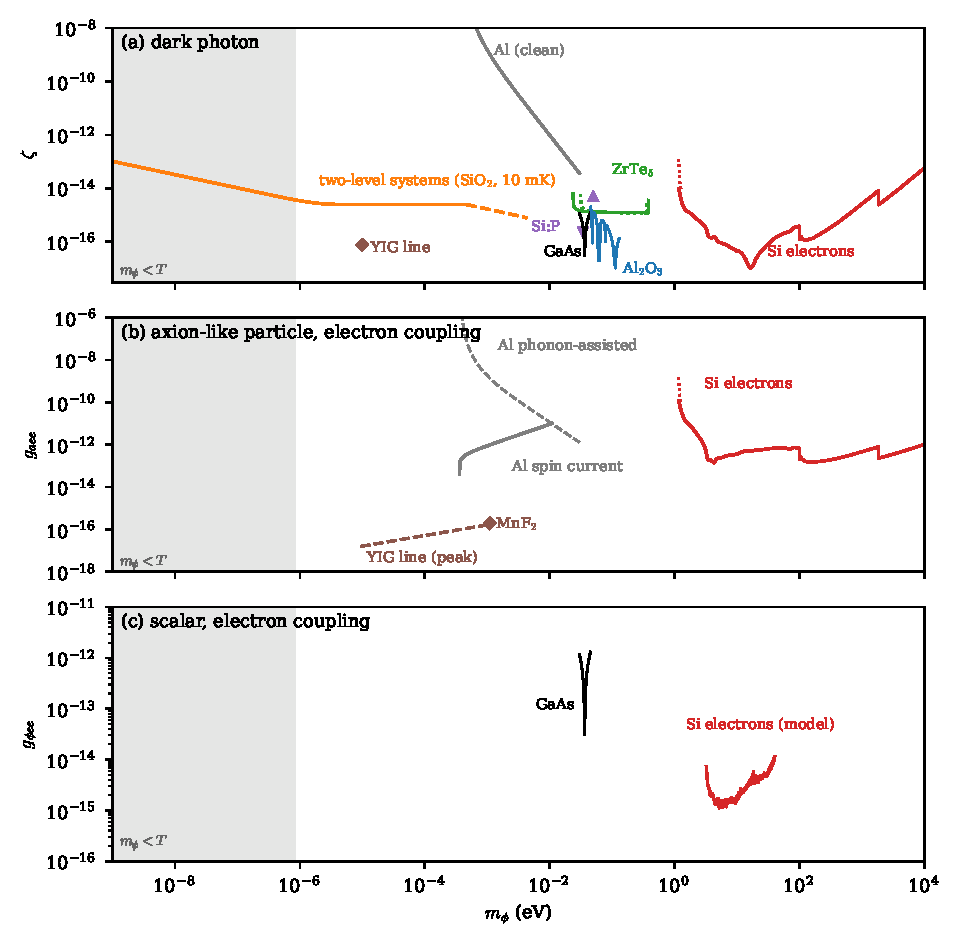
\includegraphics[width=0.86\linewidth]{figures/ch17/fig17_2.pdf}
  \caption{Absorption coverage: coupling for three events in one kilogram and year without background, $\rho_\chi = \SI{0.3}{GeV.cm^{-3}}$, against the boson mass. (a) Dark photon. Two-level systems of a thermal SiO$_2$ film at \SI{10}{mK}, $\tan\delta_0 = 3\times10^{-4}$, $\varepsilon_r = 3.9$, \cref{eq:16.7-dp} (solid, up to \SI{0.46}{meV}), and the vibrational absorption of the glass up to its Ioffe--Regel frequency, \SI{4.3}{meV} (dashed; \cref{lim:16.7d}). Clean aluminum, phonon-assisted pair creation with the Debye transport function, \cref{eq:15.4-holstein}. Si:P at \SI{e15}{cm^{-3}}: the $2p_0$ line at \SI{34.11}{meV} (down triangle) and the continuum at \SI{50}{meV} (up triangle), \cref{sec:16.5-absorption}. ZrTe$_5$ with the background in the total $\varepsilon$, polarization average, measured-structure (solid) and relaxed-cell (dotted) parameters of \cref{fig:16-zrte5}. GaAs and sapphire single-phonon lines, widths of \cref{fig:11-dpabs}. Silicon electrons from measured optical constants at \SI{300}{K} from \SI{1.1728}{eV}, with the cold excitonic edge of \cref{eq:13.8-edge} dotted up to \SI{1.3}{eV}. Diamond-shaped point: the Kittel line of a YIG sphere at \SI{10}{\micro eV}, vacuum $\zeta$, polarization random. (b) Axion-like particle, electron coupling. YIG Kittel line on resonance as it is tuned from \SI{9.5}{\micro eV} to \SI{1.16}{meV} (\SI{10}{T}), \cref{eq:14.3-peak}, and the MnF$_2$ resonance at \SI{1.1}{meV} (diamond-shaped point), both with the assumed width $\varGamma_{\mathrm{M}} = 10^{-5}\omega$. Clean aluminum: direct pair creation by the spin current, \cref{eq:15.4-sJ} with the quasiparticle factor $1/(1 + \lambda_{\mathrm{ep}}) = 0.70$, up to \SI{10.9}{meV} (solid), and the phonon-assisted $\sigma_1$ that published projections use (dashed). Silicon electrons from the measured $\sigma_1$, \cref{eq:10.7-alp}. (c) Scalar, electron coupling: the GaAs phonon line with the site couplings of \cref{eq:11.8-G}, and the kinetic-energy row of silicon in the empirical-pseudopotential model of \cref{fig:10-absorption}. Gray: $m_\phi < T$ for $T = \SI{10}{mK}$, where counting has lost its advantage over a coherent readout (\cref{sec:17.2-coherent}).}
  \label{fig:17-abs-coverage}
\end{figure}

\begin{table}[tbp]
  \centering
  \caption{Absorbing targets of the preceding chapters by decade of boson mass, with the best reach of each, three events in a kilogram and year without background. Lines are narrow and cover one mass unless tuned; continua cover the whole range given. A dash means no target in the book absorbs that boson at leading order in that decade.}
  \label{tab:17-abs-decades}
  \small
  \begin{tabular}{@{}>{\raggedright\arraybackslash}p{0.12\linewidth}>{\raggedright\arraybackslash}p{0.37\linewidth}>{\raggedright\arraybackslash}p{0.27\linewidth}>{\raggedright\arraybackslash}p{0.14\linewidth}@{}}
    \toprule
    $m_\phi$ & dark photon, $\zeta$ & axion-like, $g_{aee}$ & scalar, $g_{\phi ee}$ \\
    \midrule
    \SI{1}{neV}--\SI{1}{\micro eV} & two-level systems, $\gtrsim 3\times10^{-15}$; acoustic modes of bodies (\cref{sec:11.8-bar}); coherent readout & --- (nuclear spins couple through $g_{aNN}$, \cref{sec:14.6}) & resonant masses (\cref{sec:11.8-mass}) \\
    \SI{1}{\micro eV}--\SI{0.1}{meV} & two-level systems, $2.4\times10^{-15}$; YIG line, $7.6\times10^{-17}$ at \SI{10}{\micro eV} (vacuum $\zeta$) & YIG line, $1.6\times10^{-17}$ at \SI{10}{\micro eV} & --- \\
    \SIrange{0.1}{1}{meV} & two-level systems to \SI{0.46}{meV}, then glass vibrations; aluminum from \SI{0.36}{meV}, $1.5\times10^{-9}$ & YIG line, $1.7\times10^{-16}$ at \SI{1.16}{meV}; aluminum, $6.1\times10^{-13}$ & --- \\
    \SIrange{1}{10}{meV} & glass vibrations to \SI{4.3}{meV}, $7.6\times10^{-16}$ & MnF$_2$ line, $1.9\times10^{-16}$ at \SI{1.1}{meV}; aluminum, $9.1\times10^{-12}$ at \SI{10}{meV} & --- \\
    \SIrange{10}{100}{meV} & GaAs line, $2.9\times10^{-17}$; Si:P $2p_0$, $2.3\times10^{-16}$; ZrTe$_5$ from \SI{23.6}{meV}, $1.25\times10^{-15}$ & --- (nucleon coupling: \cref{sec:11.6}) & GaAs line, $3.1\times10^{-14}$ \\
    \SIrange{0.1}{1}{eV} & sapphire, $1.0\times10^{-17}$ at \SI{112}{meV}; ZrTe$_5$ to \SI{0.38}{eV}; none from \SIrange{0.38}{1.17}{eV} & --- & --- \\
    \SIrange{1}{10}{eV} & silicon from \SI{1.1728}{eV}; $4.4\times10^{-17}$ at \SI{10}{eV} & silicon, $1.4\times10^{-13}$ at \SI{4.3}{eV} & silicon (model), $1.1\times10^{-15}$ \\
    \SIrange{10}{100}{eV} & silicon plasmon, $1.0\times10^{-17}$ at \SI{16.4}{eV} & silicon, $3$--$5\times10^{-13}$ & silicon (model) \\
    \SIrange{0.1}{10}{keV} & silicon, $1.9\times10^{-16}$ at \SI{100}{eV}, $2.6\times10^{-15}$ at \SI{1}{keV} & silicon to \SI{1}{keV}, $3$--$5\times10^{-13}$ & --- \\
    \bottomrule
  \end{tabular}
\end{table}

The dark photon is covered almost everywhere, with two weak stretches. Between \SI{0.38}{eV}, where the Dirac cone of ZrTe$_5$ ends at twice its cutoff, and \SI{1.17}{eV}, where cold silicon begins to absorb, no target of the book absorbs at leading order; the sapphire lines and their multiphonon background end near \SI{0.12}{eV}. A narrow-gap semiconductor or a Dirac material with a wider cone would fill this gap, with the screening ceiling of its background constant. The second weak stretch is the meV decade, where the glass absorbs through its disordered vibrations at $\zeta \approx 10^{-15}$ and the superconductor is screened out.

The axion-like particle with its electron coupling has fewer targets. Magnons cover \SI{10}{\micro eV} to a meV, as far as a laboratory field tunes their lines; clean aluminum covers \SI{0.36}{meV} to \SI{11.5}{meV}, above which its phonon-assisted absorption takes over; and silicon covers everything above its edge that the tables reach. Between \SI{10}{meV} and \SI{1.17}{eV}, however, no target of the preceding chapters covers this coupling. Phonons absorb an axion-like particle through its nucleon coupling alone, on the spin-carrying isotopes of a crystal (\cref{sec:11.6}), and a Dirac material would need its spin-current response computed with its strong spin--orbit coupling, which the factor $\frac34$ of \cref{eq:10.7-alp} does not contain. The scalar has two targets: the GaAs phonon line, suppressed by the near-cancellation of its sublattices, and the kinetic row of silicon above its direct gap, which in \cref{fig:17-abs-coverage}c is a model with pseudo-wavefunctions. Between the indirect edge and \SI{3.1}{eV} silicon absorbs a scalar only with a phonon, through the kinetic row of \cref{sec:13.8}, which no measurement provides.

A tuned line and a continuum are compared differently. On resonance the Kittel line of YIG reaches $g_{aee} = 1.6\times10^{-17}$ at \SI{10}{\micro eV}, but only within its full width $\varGamma_{\mathrm{M}} = 10^{-5}m_\phi$. A search that scans the line across one e-fold of mass with uniform exposure spends a fraction $(\pi/2)\varGamma_{\mathrm{M}}/m_\phi = 1.6\times10^{-5}$ of its time on each mass. Averaged over the scan the reach is $4.1\times10^{-15}$, still a hundred times better than the continuum of clean aluminum at its best mass. The MnF$_2$ resonance at \SI{1.1}{meV} gives $1.9\times10^{-16}$ on resonance and $4.8\times10^{-14}$ averaged. The peak values rest on the assumed ratio $\varGamma_{\mathrm{M}}/\omega = 10^{-5}$ (\cref{sec:14.3}). The averaged ones do not depend on it, since the area of the line, not its height, sets what a scan delivers, as for the phonon lines of \cref{eq:11.8-Rint}. The fixed lines of GaAs, sapphire and Si:P cover their own masses alone.

\begin{workedexample}{The handover from GaAs phonons to silicon electrons}\label{we:17-handover}
GaAs absorbs a dark photon at its longitudinal optical phonon, \SI{36.35}{meV}, with all the weight of the line, $\mathcal{I}_{\mathrm{pol}} = \SI{0.759}{meV}$, within a few widths, and with multiphonon absorption up to a few phonon energies. Its electrons absorb from its gap, \SI{1.52}{eV} at low temperature (\cref{sec:3.3}). Silicon absorbs from its excitonic edge. At which mass does silicon take over?

\emph{The phonon line does not decide it.} The damped factorized model of \cref{fig:11-dpabs} gives $\varepsilon_2 = 2.5\times10^{-4}$ at \SI{1.17}{eV}, an absorption coefficient of \SI{4.3}{cm^{-1}} with the refractive index 3.48 used below. That value is an artifact of the model: with different widths in its numerator and denominator it tends to $\varepsilon_2 = \varepsilon_\infty(\gamma_{\mathrm{L}} - \gamma_{\mathrm{T}})/\omega$ far above the line, a constant conductivity. A Lorentz oscillator with a single width gives $\varepsilon_2 = 4.8\times10^{-7}$ and \SI{0.008}{cm^{-1}} at the same energy. A pure crystal transmits there, and what it absorbs depends on its defects.

\emph{Equal rates.} Per unit mass the rates are equal when $L_{\mathrm{GaAs}}/\rho_{\mathrm{GaAs}} = L_{\mathrm{Si}}/\rho_{\mathrm{Si}}$. Below a gap $\varepsilon_2 \ll \varepsilon_1 = n_r^2$, and with $\varepsilon_2 = n_r\alpha_{\mathrm{abs}}/\omega$ the loss function is $L = \alpha_{\mathrm{abs}}/(n_r^3\omega)$. With $n_r = 3.48$ for GaAs at \SI{22}{\celsius}, from the dispersion formula of Skauli et al.~\cite{skauli2003improved} as tabulated in Ref.~\cite{polyanskiy2024refractiveindex}, $n_r = 3.56$ for silicon at \SI{300}{K}~\cite{franta2017temperature}, and densities 5.361 and \SI{2.33}{g.cm^{-3}}, GaAs needs $(3.48/3.56)^3\times5.361/2.33 = 2.15$ times the absorption coefficient of silicon to match it.

\emph{The silicon edge.} At millikelvin temperatures silicon absorbs from the $1s$ replica of the transverse acoustic branch, $\Eg(0) + \omega_{\mathrm{TA}} - E_x^b = \SI{1.17277}{eV}$, and \cref{eq:13.8-edge} rises there as a square root. With the scale of \cref{sec:13.8},
\begin{equation*}
  \alpha_{\mathrm{abs}}^{\mathrm{Si}} = \SI{13.3}{cm^{-1}}\,\bigl[(m_\phi - \SI{1.17277}{eV})/\mathrm{eV}\bigr]^{1/2} ,
\end{equation*}
which is \SI{0.13}{cm^{-1}} at \SI{0.1}{meV} above the threshold and \SI{0.42}{cm^{-1}} at \SI{1}{meV}.

\emph{The handover.} Setting $2.15\,\alpha_{\mathrm{abs}}^{\mathrm{Si}}$ equal to the absorption of the GaAs crystal places the handover \SI{0.012}{meV} above the threshold for \SI{0.1}{cm^{-1}} and \SI{1.2}{meV} above it for \SI{1}{cm^{-1}}. A crystal absorbing \SI{10}{cm^{-1}} would move it \SI{40}{meV} up; at that distance the further replicas of \cref{eq:13.8-edge} have opened, and the square-root onset alone would have put it at \SI{0.12}{eV}. For any GaAs crystal transparent to better than \SI{1}{cm^{-1}}, silicon takes over within a meV of its excitonic edge, at $m_\phi \simeq \SI{1.173}{eV}$, and the square-root onset of the replica makes the handover sharp. A meV above the threshold silicon reaches $\zeta = 5.6\times10^{-14}$, two thousand times weaker than the GaAs line at its center.
\end{workedexample}

The worked example uses a model of the cold edge. The cold measurements near the edge differ among themselves by a factor of twenty (\cref{sec:13.8}), which moves the absorption of silicon but not the place of the handover, since the threshold is fixed by the gap, the phonon and the exciton binding.

\subsection{Coherent and counting readout}\label{sec:17.2-coherent}

A YIG sphere tuned to \SI{10}{\micro eV} counts the quanta it absorbs (\cref{we:14-yig}). A $^{207}$Pb sample at \SI{1}{neV} reads the transverse magnetization that the field drives (\cref{sec:14.6}). Both measure the absorptive part of a response near $\omega = m_\phi$, but the first counts quanta of energy $m_\phi$ and the second measures the amplitude of a field. Which readout is better at a given mass depends on the thermal occupation $n_{\mathrm{B}}(m_\phi) = 1/(\ee^{m_\phi/T} - 1)$ of the mode that is read, with $T$ the temperature of that mode.

Take a record of length $t_{\mathrm{int}}$ longer than the coherence time. The signal is spread over $N_{\mathrm{coh}} \simeq t_{\mathrm{int}}\Delta\omega_{\mathrm{eq}}/2\pi$ independent frequency bins, with $\Delta\omega_{\mathrm{eq}} = 2.67/t_{\mathrm{coh}}$ the equivalent width of the line (\cref{sec:14.6-stats}), and it delivers $\bar N_{\mathrm{sig}}$ absorbed quanta. A counter whose detection band is the line sees, in the same bins, $\bar N_{\mathrm{th}} = n_{\mathrm{B}}(m_\phi)N_{\mathrm{coh}}$ thermal quanta. They are chaotic, and their number fluctuates with the variance $\bar N_{\mathrm{th}} + \bar N_{\mathrm{th}}^2/N_{\mathrm{coh}} = N_{\mathrm{coh}}n_{\mathrm{B}}(m_\phi)[n_{\mathrm{B}}(m_\phi) + 1]$ of \cref{sec:14.6-regime}. A linear readout, a phase-preserving amplifier or a magnetometer, measures both quadratures of the mode, and its noise is at least $n_{\mathrm{B}}(m_\phi) + 1$ quanta per bin: the thermal quanta plus one zero-point quantum, half of it present at the input and half added by the amplifier~\cite[Eq.~(9)]{lamoreaux2013analysis}. This per-bin noise has the rms $n_{\mathrm{B}}(m_\phi) + 1$, and summed in quadrature over the bins it fluctuates by $[n_{\mathrm{B}}(m_\phi) + 1]N_{\mathrm{coh}}^{1/2}$. The significance of the signal is then $\bar N_{\mathrm{sig}}/\{N_{\mathrm{coh}}n_{\mathrm{B}}(m_\phi)[n_{\mathrm{B}}(m_\phi) + 1]\}^{1/2}$ for the counter and $\bar N_{\mathrm{sig}}/\{N_{\mathrm{coh}}^{1/2}[n_{\mathrm{B}}(m_\phi) + 1]\}$ for the linear readout, whose square is the weak-signal statistic $\mathsf{t}$ of \cref{sec:14.6-stats} with $x_k = \bar N_{\mathrm{sig}}/\{N_{\mathrm{coh}}[n_{\mathrm{B}}(m_\phi) + 1]\}$ in each bin. At equal significance the counter needs fewer signal quanta by the ratio
\begin{keyresult}[Counting against linear readout]
\begin{equation}
  \frac{\bar N_{\mathrm{sig}}^{\mathrm{lin}}}{\bar N_{\mathrm{sig}}^{\mathrm{cnt}}} = \Bigl[\frac{n_{\mathrm{B}}(m_\phi) + 1}{n_{\mathrm{B}}(m_\phi)}\Bigr]^{1/2} = \ee^{m_\phi/2T} ,
  \label{eq:17.2-ratio}
\end{equation}
for the same absorber, record and line, as long as the counter sees thermal quanta in the record and its detection band is the line width $\Delta\omega_{\mathrm{eq}}$. A counter that sees a band $B$ wider than the line collects more thermal quanta, and the ratio is multiplied by $(B/\Delta\omega_{\mathrm{eq}})^{-1/2}$. In the coupling, which enters the signal squared, the ratio is $\ee^{m_\phi/4T}$. For $n_{\mathrm{B}}(m_\phi) \ll 1$ the Poisson treatment of Lamoreaux and collaborators~\cite[Eqs.~(12)--(14)]{lamoreaux2013analysis} is the limit of this result; their cavity counter sees the whole cavity band, which carries the extra factor $(Q_{\mathrm{c}}/2\pi Q_a)^{1/2}$ of their Eq.~(18), with $Q_{\mathrm{c}}$ and $Q_a$ the quality factors of the cavity and of the line.
\end{keyresult}

Three regimes follow. For $m_\phi \ll T$ the ratio tends to one. Each mode holds many thermal quanta, their fluctuation dominates either readout, and a counter gains nothing over a measurement of the field, while it would have to resolve single quanta far below the thermal energy. At \SI{1}{neV} a mode at \SI{4.2}{K} holds $3.6\times10^5$ quanta and one at \SI{10}{mK} holds 861, and every search there reads the field. For $m_\phi \approx T$ the gain is modest, 1.65 in the signal and 1.28 in the coupling at $m_\phi = T$. For $m_\phi \gg T$ the counter wins exponentially, until the record holds no thermal quantum at all. Requiring zero thermal counts with \SI{95}{\percent} probability, $\bar N_{\mathrm{th}} < 0.05$, the counter needs three signal quanta (\cref{sec:1.5})~\cite[Eqs.~(19), (20)]{lamoreaux2013analysis}, whatever the mass. With $\Delta\omega_{\mathrm{eq}} = 2.67\,m_\phi v_0^2$ this happens above \SI{17}{\micro eV} for a one-hour record and \SI{20}{\micro eV} (\SI{4.9}{GHz}) for one day at \SI{10}{mK}, and above \SI{0.19}{meV} and \SI{0.22}{meV} at \SI{100}{mK}, that is, at $m_\phi \approx (20$--$26)\,T$. The linear readout still needs $\bar N_{\mathrm{sig}} = (2.71\,N_{\mathrm{coh}})^{1/2}[n_{\mathrm{B}}(m_\phi) + 1]$ at the threshold $\mathsf{t} = 2.71$ of \cref{eq:C.14-thresholds}, the one-sided \SI{95}{\percent} level. For instance, at \SI{24.8}{\micro eV}, the 6-GHz mass of \cref{we:16-tls-dp}, a day at \SI{10}{mK} spreads the line over $8.7\times10^8$ bins, and the linear readout needs $4.9\times10^4$ quanta against the counter's three, a factor of 127 in the coupling. At \SI{10}{\micro eV} the same record still holds 3200 thermal quanta, and the counter wins by 330 in the signal and 18 in the coupling.

The gray band of \cref{fig:17-abs-coverage}, $m_\phi < T$ (\SI{0.86}{\micro eV}, or \SI{210}{MHz} at \SI{10}{mK}), is where the advantage of counting has fallen below $\ee^{1/2}$ and tends to one, and the field is read coherently. Above that mass the counter gains $\ee^{m_\phi/4T}$ in the coupling, and above $20\,T$ it is limited by the absorbed quanta alone, with a reach that improves as $t_{\mathrm{int}}^{-1/2}$ against the $(t_{\mathrm{int}}t_{\mathrm{coh}})^{-1/4}$ of the field measurement (\cref{eq:14.6-scaling}). Two effects reduce the advantage. A linear readout of one quadrature of a squeezed mode can go below one zero-point quantum~\cite{lamoreaux2013analysis}, which narrows the gap by the degree of squeezing. A real counter, moreover, has dark counts besides the thermal quanta, and they add to its background. The background-free counting that the reach curves of \cref{fig:17-abs-coverage} assume holds where both are absent.
